%%aquapod with flippers
\begin{figure}[tb]
  \centering
  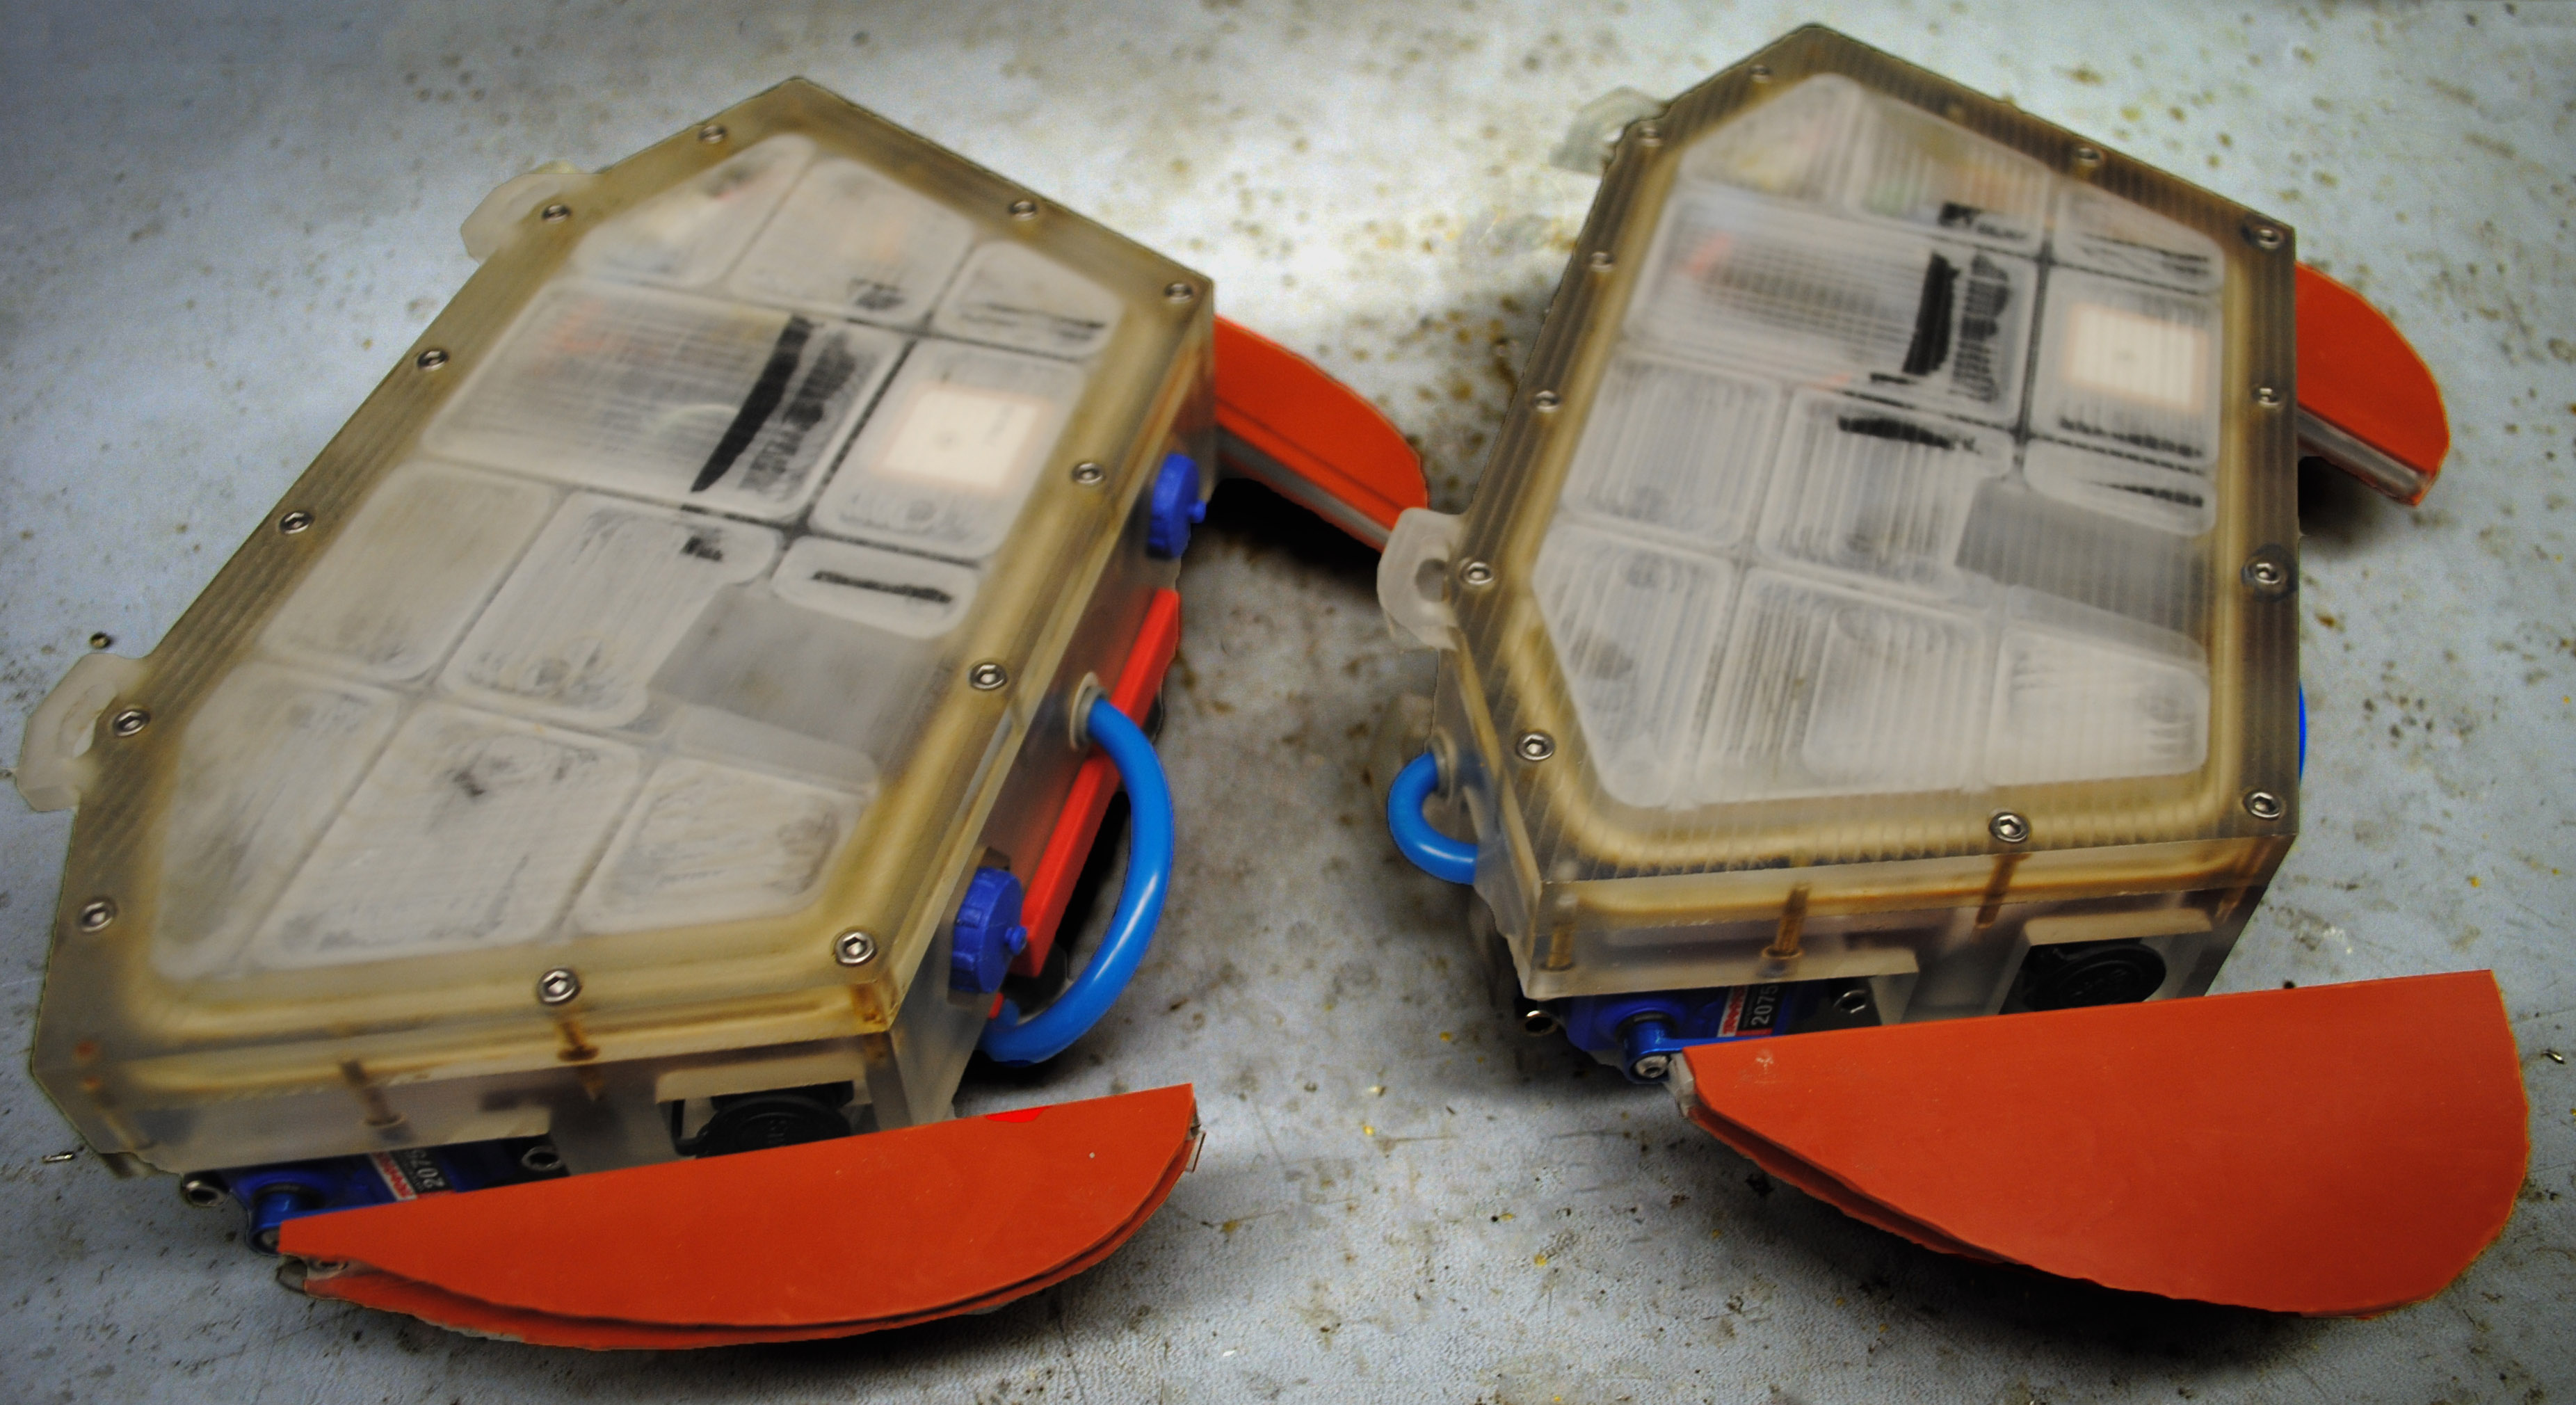
\includegraphics[width=1\columnwidth]{images/aquapod_flippers.jpg}
  \vspace{-10pt}
  \caption{Aquapod with flippers}
  \vspace{-20pt}
  \label{fig:aquapod_flippers}
\end{figure}



%%aquapod at diving well  
\begin{figure}[tb]
  \centering
  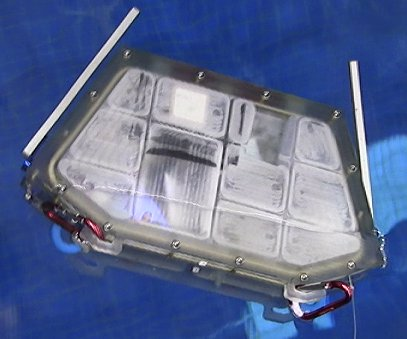
\includegraphics[width=1\columnwidth]{images/aquapod_v1_pool.jpg}
  \vspace{-10pt}
  \caption{Aquapod during diving well test}
  \vspace{-20pt}
  \label{fig:aquapod_pool}
\end{figure}




%Mobile robots are often proposed as a favorable substitute to human correspondence in emergency response, disaster relief, and environmental monitoring scenarios.  In this work, the next iteration of the Aquapod is proposed as a method to facilitate collection of subsurface liquid samples in order to assess toxicity levels in a body of water.  This amphibious small form-factor robot is equipped with a buoyancy control unit, detachable fluidic sampling unit, and a wide range of sensing and processing capabilities.  The robot was designed to move and collect water samples to a maximum depth of ten meters.  Its unique form of tumbling locomotion results in a versatile platform that can be used in both terrestrial and aquatic environments leveraging its high mobility-to-size ratio.

\subsection{The Aquapod}


The Aquapod is an amphibious robot capable of traversing land by carrying out subsequent tumbles on land and on the bottom of a body of water. It builds upon the Adelopod \cite{Hemes2009} and \cite{Carlson2011} in order to enable additional capabilities.  The Aquapod is intended as a method to facilitate collection of subsurface liquid samples in order to assess toxicity levels in a body of water. Employing a buoyancy control system allows it to alter its density and go from an initial positively buoyant state to neutral buoyancy and negative buoyancy as needed.


This small form-factor amphibious robot is also equipped with a detachable fluidic sampling unit, and a wide range of sensing and processing capabilities in order to carry out a number of environmental monitoring tasks, such as the collection of subsurface liquid sample collection.  It is designed to withstand internal and external hydrostatic pressures of more than ten meters. Its unique form of tumbling locomotion results in a versatile platform that can be used in both terrestrial and aquatic environments leveraging its high mobility-to-size ratio.


%%%%%%%%%%%%%%%%%%%%%%%%%%%%%%%%%%%%%%%%%%%%%%%%%%%%%%%%%
\subsubsection{Introduction}


The Aquapod 1.0 (or ``Aquapod") described in this paper takes its inspiration from the RC Aquapod~\cite{Carlson2011}, revising the design and extending the intended capabilities of this prototype.  The RC Aquapod, in turn, stems from the Adelopod~\cite{Hemes2011}, using the concept of tumbling for ground locomotion.  However, the Aquapod family adds the ability to function in aqueous environments, both on the surface and underwater, using a buoyancy control system to affect its vertical position in the water.  The buoyancy control is a static alternative to dynamic diving systems used in some submersibles, proving to be more energy efficient to control the robot's depth by only requiring energy to change diving characteristics like sinking or floating~\cite{Detweiler2009}.  This was present in the RC Aquapod, but was revised and developed in more detail for this application.
%----------------------------------------------------------------------------------------------------------------------------------------------------------
 

%%%%%%%%%%%%%%%%%%%%%%%%%%%%%%%%%%%%%%%%%%%%%%%%%%%%%%%%%
\subsection{ Mechanical Design}\
Over the course of the project, the mechanical design of almost every component was revisited and revised to expand capabilities and design for the environment of a marshland.  It was estimated that the ``shallow water" environment that the Aquapod was to be used in would not exceed 10 meters: therefore, the Aquapod was designed to reliably withstand pressures seen at that depth.  Additionally, energy efficiency was an important design criteria to ensure a safe recovery of the robot, thus the Aquapod uses a peristaltic pump and a bladder to ingest surrounding water to alter its buoyancy.  This system was present in the RC Aquapod, but was revised and developed in more detail to meet the specified design requirements, notably the chemical compatibility of components that interact with the environment.  

The outer shell of the Aquapod is made out of clear polycarbonate, which meets both the stress requirements for diving to 10 meters and is chemically compatible with materials that the Aquapod is expected to encounter.  Among the major challenges and additions to the Aquapod design, is the new sealing methodology including all connections and seams in the hull--which encloses the electronics, the revision of the Buoyancy Control Unit (BCU), the revisited drive system for the arms, as well as the addition of an external water sampling module attaching directly to the outer hull of the robot. See Figure \ref{fig:annotated_aquapod} for a diagram of the internal components.

\begin{figure}[htb]
    \centering
    %\includegraphics[width=.90\columnwidth]{../images/Aquapod2-Mod.png}
    \includegraphics[width=.90\columnwidth]{images/Aquapod2-Mod.png}
    \caption{ Aquapod components}
    \vspace{-20pt}
    \label{fig:annotated_aquapod}
\end{figure}

	\subsubsection{Sealing}
		In order for the Aquapod to be capable to descend to designed depth, all locations susceptible to fluid ingression were designed to withstand a maximum hydrostatic gauge pressure of approximately 14 psi\(_g\), double that of atmospheric pressure. 
	
% Main seal
		The seal formed between the top and bottom halves of the hull, the main seal, is formed by compression of an O-ring. This seal was designed to be hermetic and withstand the maximum design pressure.  Empirical results found this particular seal to have greater performance over alternate designs, including the flat-gasket design of the RC Aquapod.
            
%aquapod deepwater render with callout (aquapod2_mod, fig:annotated_aquapod)

		One of the main advantages of the O-ring and gland design was lower force requirements to form an effective seal than other designs. This is advantageous because the seal is highly dependent on the compressive force exerted between the hull halves, however, the maximum force that was exertable is a function of the stress that the material and fastening method allow. Polycarbonate was chosen for the hull material and the hulls were fastened by a set of screws on the periphery of the Aquapod, therefore minimal compression force requirements were necessary to prevent stripping out the threads of the tapped holes.

		Another advantage of the O-ring is that it forms a more robust seal as its circular cross-section provides a sealing profile that commences with linear contact and progresses to an area as the O-ring is compressed. This initial linear contact is desirable because it concentrates greater sealing pressure at the onset of the sealing phase. The alternative gasket design, required special features, such as a tooth, to be incorporated into the hull, to form an effective seal.  This method presented its own challenges, as high compressive forces were required, but over compression can lead to rupture of the gasket. 

		Other locations that were susceptible to fluid ingression include various ports, power components, the external motors, and lines that provided power and communication to the external motors. The pressure sensor port is press-fit into the hull and sealed in conjunction with a tetrachloroethylene-based marine sealant and adhesive (herein referred to simply as sealant). The Aquapod sports two commercial-off-the-shelf (COTS) mini-USB panel-mounted ports for data I/O as well as for programming.  These ports are desirable as compatible hardware is easily found and convenient. The ports are Ingress Protection 68 (IP68) rated and were modified to extend their sealing capabilities to meet our specification requirements. 

 		The power switch is a double-pole double-throw three position micro-switch with a rubber boot to ensure hermeticity. Power components include the on/off switch and the charging ports, these were COTS and were implemented in the design with no further modifications. 

		The control and power buses for the arms and the sampler module servos, are routed through flexible PVC tubing in order to take advantage of industry standard pneumatic push-to-connect (PTC) fittings.  The PTC fittings form a hermetic seal with the tubing and their design prevents accidental disconnection by unexpected tension, e.g.\ when a twig or other obstacle become caught on the tubing. The sealing of the external motors will be described in Section \ref{arm_motors} below. 

	\subsubsection{Buoyancy Control Unit}
		The BCU is largely similar to the one used in the RC Aquapod. It is comprised of a bladder, gearmotor, and pumphead.  The current iteration of the BCU has seen the addition of an encoder for angular velocity feedback as well as a motor specified to meet greater torque and angular velocity requirements while also meeting weight and volumetric constraints.  Additionally, the stock tubing in the pumphead was replaced with one that offers high chemical compatibility with fluids which it could potentially contact while minimizing the hardness of the tube to achieve higher flowrates. 

	\subsubsection{Chemical Compatibility}
		 The Aquapod was intended as a tool to assist in environmental monitoring, therefore, the hull, main seal, and all other surfaces exposed to the potential chemical-laden environments need to be chemically compatible with substances that may negatively impact their properties. A short list of fluids that were taken into account consist of fresh water, salt water, crude oil, gasoline, diesel fuel, and fuel oils.
		  
		  A material's chemical compatibility was one of the most important factors when choosing components that would be in contact with external fluids. The severity of foreign chemicals on the elastomeric components is a function of concentration as well as time with the main consequences being swelling or stiffening of the elastomers.
	
		The bladder, O-ring, and tubing were the components most susceptible to chemical degradation, therefore the selection of these components was in large part driven by compatibility constraints. The O-ring is made of a formulation of Viton\textsuperscript{\textregistered} that is compatible with the aforementioned fluids and has 40 Shore A hardness which creates a better seal in low pressure applications \cite{Parker-Hannifin2007}.
	
		The pump is one of the components that is most susceptible to the potential degradation due to the elastomeric tubing which forms part of its design and serves to transport fluids. These fluids originate exterior to the Aquapod and are potential carriers of chemicals that can degrade the tubing. The peristaltic pumphead constrains and squeezes sections of tubing to provide fluid displacement. Chemical degradation can aggravate the significant stress already imparted on the tubing mechanically and lead to premature failure.  
	
		Tubing hardness is important as the flowrate is inversely proportional to the tubing hardness. The silicone tubing that comes stock with the pumphead offers a favorable flowrate; however, due to its poor chemical compatibility, it was replaced with unreinforced high-flex white PVC.  The PVC tubing meets chemical compatibility constraints and has approximately the same hardness as the stock silicone tubing. 
		
	\subsubsection{Arm Powertrain}
	\label{arm_motors}
		The Aquapod's powertrain is found completely external to the hull and consists of a set of motors on the underside of the robot that are coupled to a pair of aluminum arms. The Aquapod moves by driving arms to execute end-over-end tumbles. To achieve forward motion on flat terrain, the arms move in unison in the same direction, however, in order to move in nonuniform terrain or other types of movements it was desirable to exploit the differential nature of the powertrain. Situations arise in which, due to the terrain, or the required type of movement only one arm is used to move the robot.  Therefore it was necessary to specify the powertrain to meet scenarios in which the Aquapod's weight relies solely on one arm and motor. 
		
		The geometry of the Aquapod's arms were driven primarily by the need to support the full weight of the Aquapod (approximately 2.65 lbs) to enable effective tumbling. Material selection was important in choosing a material of low weight and high resistance to corrosion in marine environments, as well as meet the chemical compatibility requirements from the previous section. 

		The Aquapod's arms are driven by high torque servomotors that have been modified for hermeticity and continuous rotation. Enabling continuous rotation from an COTS servomotor required mechanically altering the output gear of the geartrain, replacing the stock circuitry with an analog absolute encoder capable of providing an analog output for continuous position feedback, and providing control via the onboard embedded system. 
		
		Ensuring hermeticity after arm motor modifications presented multiple sealing challenges.  The motors' stock configuration features a rubber grommet that routes three wires through its exterior housing.  In light of the addition of the encoder, it was necessary to route two additional wires through the shell, bringing the total to five.  The wires are routed inside soft PVC tubing which acts as the new grommet. Routing the power and control buses in tubing also allows an effective seal using the PTC fittings found on the hull. Additionally, using a combination of tubing and fittings allows the arm servos to be easily replaced. The new grommet and the seams present throughout the exterior motor housing are further sealed with marine sealant.  

	The most critical seals of the Aquapod are located at the output shafts of the arm motors as these seals are dynamic in nature. Being dynamic they require a seal to be kept when the powertrain is in motion. The motor's stock configuration contains a bearing and O-ring that are mounted on the output shaft of the arm servo. The bearing serves to align the output shaft and the O-ring to form a seal with the exterior motor housing. To improve seal pressure the stock O-ring was replaced with a thicker and softer Buna-N O-ring. Additionally, exterior to the motor housing, an O-ring was added to form a secondary seal when compressed between the external housing and the arm. 	

	\subsubsection{Sampler Design}
		 The sampler module was designed and created for the Aquapod in order to capture water samples and bring them to the surface. Equipment utilized to carry out substance detection methods are not practical in miniature robots, therefore, collecting these samples is valuable. Furthermore, a more thorough analysis of the samples can be done in a laboratory setting.

Figure~\ref{fig:sampler} shows a rendering of the sampler module which attaches to the backside of the Aquapod.  The module is designed with energy efficiency in mind to prolong battery life: thus, two caps on each end of a tube are held closed by an elastic band requiring no electric power to remain closed.  A servo is engaged only to open each end and take the sample, then released to close the vials again.  The caps are padded with a rubber surface, while the tubes have been filed to a sharper end to promote higher pressure between the tube and the caps (by reducing the contact area) and thus more effectively sealing the vial.

The current model has two vials, each opened by its own servomotor.  The motors themselves required additional modifications to survive the maximum design pressure: marine sealant was applied to each seam in the plastic body, a thicker O-ring was placed on the shaft of the servo to seal it, and the circuitry inside the servo was covered in epoxy. This substantially improved the life of these units.

A waterproof connector runs into the hull of the Aquapod to connect power and signal lines to the interior electronics.  These connectors are also injected with epoxy to ensure a waterproof connection.  The backpack itself is attached to the Aquapod hull using screws for easy removal.

%Annotated sampler rendering 
\begin{figure}[htb]
	\centering
	\includegraphics[width=1\columnwidth]{images/sample_v2.jpg}
	\caption{Sampler}
	\vspace{-10pt}
	\label{fig:sampler}
\end{figure}
%-------------------------------------------------------------------------------------------

%%%%%%%%%%%%%%%%%%%%%%%%%%%%%%%%%%%%%%%%%%%%%%%%%%%%%%%%%%%%%%%%%%%%%%%%%%%%%%%%%%%%%%%%%%%%
\subsubsection{Embedded System Design}
This section presents an overview of the embedded system design of the Aquapod, which has been split into three main components. Two of the printed circuit boards (PCBs) were custom designed to meet the volume restrictions while the third PCB was a small, COTS module. Splitting the electronics into separate boards allows the design to be highly versatile and expand with minimal effort. This also allowed for different sensor suites to be interchanged and made the robot more robust to ever adapting needs.

%%%%%%%%%%%%%%%%%%%%%%%%%%%%%%%%%%%%%%%%%%%%%%%%%%%%%%%%%%%%%%%%%%%%%%%%%%%%%%%%%%%%%%%%%%%%
\subsubsection{Hardware Design}
The initial RC Aquapod had no embedded system design, and so the new iteration had to make a number of drastic changes. Due to the increase in internal components, space inside the robot was limited. A three-PCB design made up of a master board, a slave board, and a fuel-gauge board allowed the components to be broken apart and better utilize the space available. The complete system architecture can be seen in Figure \ref{fig:final-arch}.

%\begin{figure}[htc]
%finalized electrical architecture
\begin{figure}[ht]
	\begin{center}
		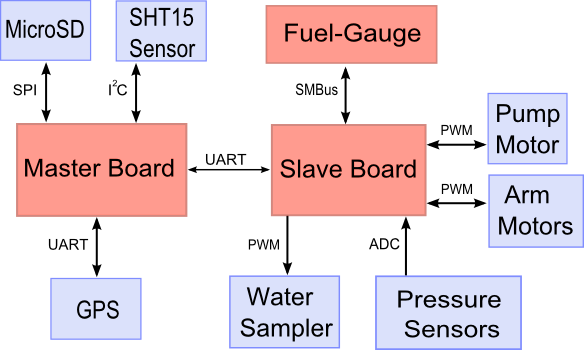
\includegraphics[width=1\columnwidth]{images/finalized-architecture2.png}
		\caption{Final embedded system architecture}
		\vspace{-20pt}
		\label{fig:final-arch}
	\end{center}
\end{figure}

%%%%%%%%%%%%%%%%%%%%%%%%%%%%%%%%%%%%%%%%%%%%%%
\subsubsection{Master Board}
In order to facilitate the requirements within the time constraints, a COTS module was used for the master board. SparkFun Electronics sells this as the Package Tracker and runs on an LPC2148 ARM7 microcontroller. This unit was chosen for its 'ready to use' mircoSD card reader, onboard sensors, and GPS interface.  The master board is responsible for controlling the state machine of the robot, making decisions, and logging the sensor data.

\subsubsection{Slave Board}
Due to the custom nature of the hardware, the slave board was designed specifically for the Aquapod robot. The main processor was chosen as the PIC16F1827 from MicroChip based on the number of required input and output pins. The slave board also includes a pressure sensor, charge recognition circuitry, communication devices, and the required motor drivers for five separate actuators (two arms, two samplers, and one pump). This board facilitates the low-level control of the motors and sensors, however, it will only act on commands sent by the master board.

%%%%%%%%%%%%%%%%%%%%%%%%%%%%%%%%%%%%%%%%%%%%%%
\subsubsection{Sensors}
The Aquapod has two absolute pressure sensors with an output range of 0.3V to 4.9V, corresponding to an input range of 3 psi\(_a\) to 42 psi\(_a\), respectively. These sensors are used to monitor internal and external pressure and act as the main decision points of the state machine.

The two arm motors feature absolute magnetic shaft encoders to report the current arm position back the slave board which handles the PID control for arm movement. The pump motor also includes a digital encoder to determine the total water volume pumped into the bladder. The sampler motors have no feedback, but operate on a standard servo open-loop signal.

The COTS master board contains a number of onboard sensors including temperature, humidity, and a 3-axis accelerometer. The board can also access the SiRF III GPS module from USGlobalSat.

By communicating with the slave board, the master board is capable of measuring and logging all of these sensor values in a central log file and can make decisions based on the returned values, this will be discussed in more detail below.
%%%%%%%%%%%%%%%%%%%%%%%%%%%%%%%%%%%%%%%%%%%%%%
\subsection{Power Architecture}
The Aquapods's power system comprises of three main parts: the battery and fuel-gauge, the battery charger, and the various power conversion electronics.  Wiring to chassis-mounted electronic components and high DC current lines is realized using twisted-pairs to increase noise immunity by reducing destructive (or unbalanced) effects resulting from electromagnetic interference coupled signals and ground return paths.

%\subsubsection{Battery and Fuel-Gauge}
%\label{sec:batt_mgmt_and_gg}
At the heart of the robot's power system is a dedicated fuel-gauging chipset, described in \cite{Kottas2009}.  It provides all the necessary features to safely monitor any lithium-ion battery chemistry's dynamics, while tracking cell (capacity) degradation over time.  The resultant smart-battery system (SBS) is compliant with SBS v1.1 standards \cite{sbs_std}, and can report a wide array of static and dynamic battery parameters while idle, charging, or discharging to a host processor - in this case, the slave and master boards. This system is shown in Figure \ref{fig:pwr_blk_diag}.

A lithium-ion polymer battery (LiPB) was chosen to power the robot.  This particular battery chemistry was selected due to its thin and light-weight packaging, high energy density and output power capabilities.  It can source roughly 14Wh of energy, and satisfies the robot's operating time requirements. 

A highly integrated LiPB switch-mode charge-management circuit is included on slave board.  It is configured to charge the LiPB pack quickly and safely and contains a pre-charge (conditioning) mode for deeply discharged batteries.

\begin{figure}%
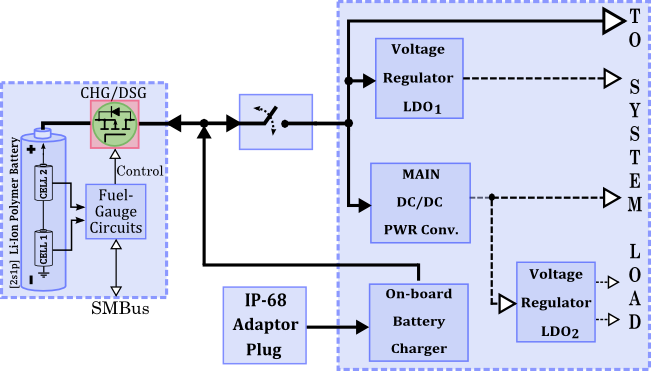
\includegraphics[width=1\columnwidth]{images/Aqua-Pod_Robot_PwrSys_Fig01.png}%
\caption{High-level power system block diagram}%
\vspace{-10pt}
\label{fig:pwr_blk_diag}%
\end{figure}

%%%%%%%%%%%%%%%%%%%%%%%%%%%%%%%%%%%%%%%%%%%%%%
\subsubsection{Communication Protocol}
Command and Acknowledgment (CMD/ACK) messages are used to exchange data and commands between the boards. This hand-shaking protocol was enforced to ensure important commands from the master board were being process and executed by the slave board before continuing with the state machine. The master board can send one command at a time in a 9-byte packet to the slave board which will execute the command or return sensor values appropriately.  
%%%%%%%%%%%%%%%%%%%%%%%%%%%%%%%%%%%%%%%%%%%%%%
\subsection{State Machine and Operational Profiles}
The main purpose for this version of the Aquapod was to collect water samples at a pre-programmed depth. Using a graphical user interface, the Aquapod can be programmed into one of four modes, including: Instant Dive(1), Remote Dive(2), Land Mode(3), and Purge Bladder(4). Selecting one of these modes will route the robot through the state machine which can be seen in Figure \ref{fig:Statemachine}.

\begin{figure}
	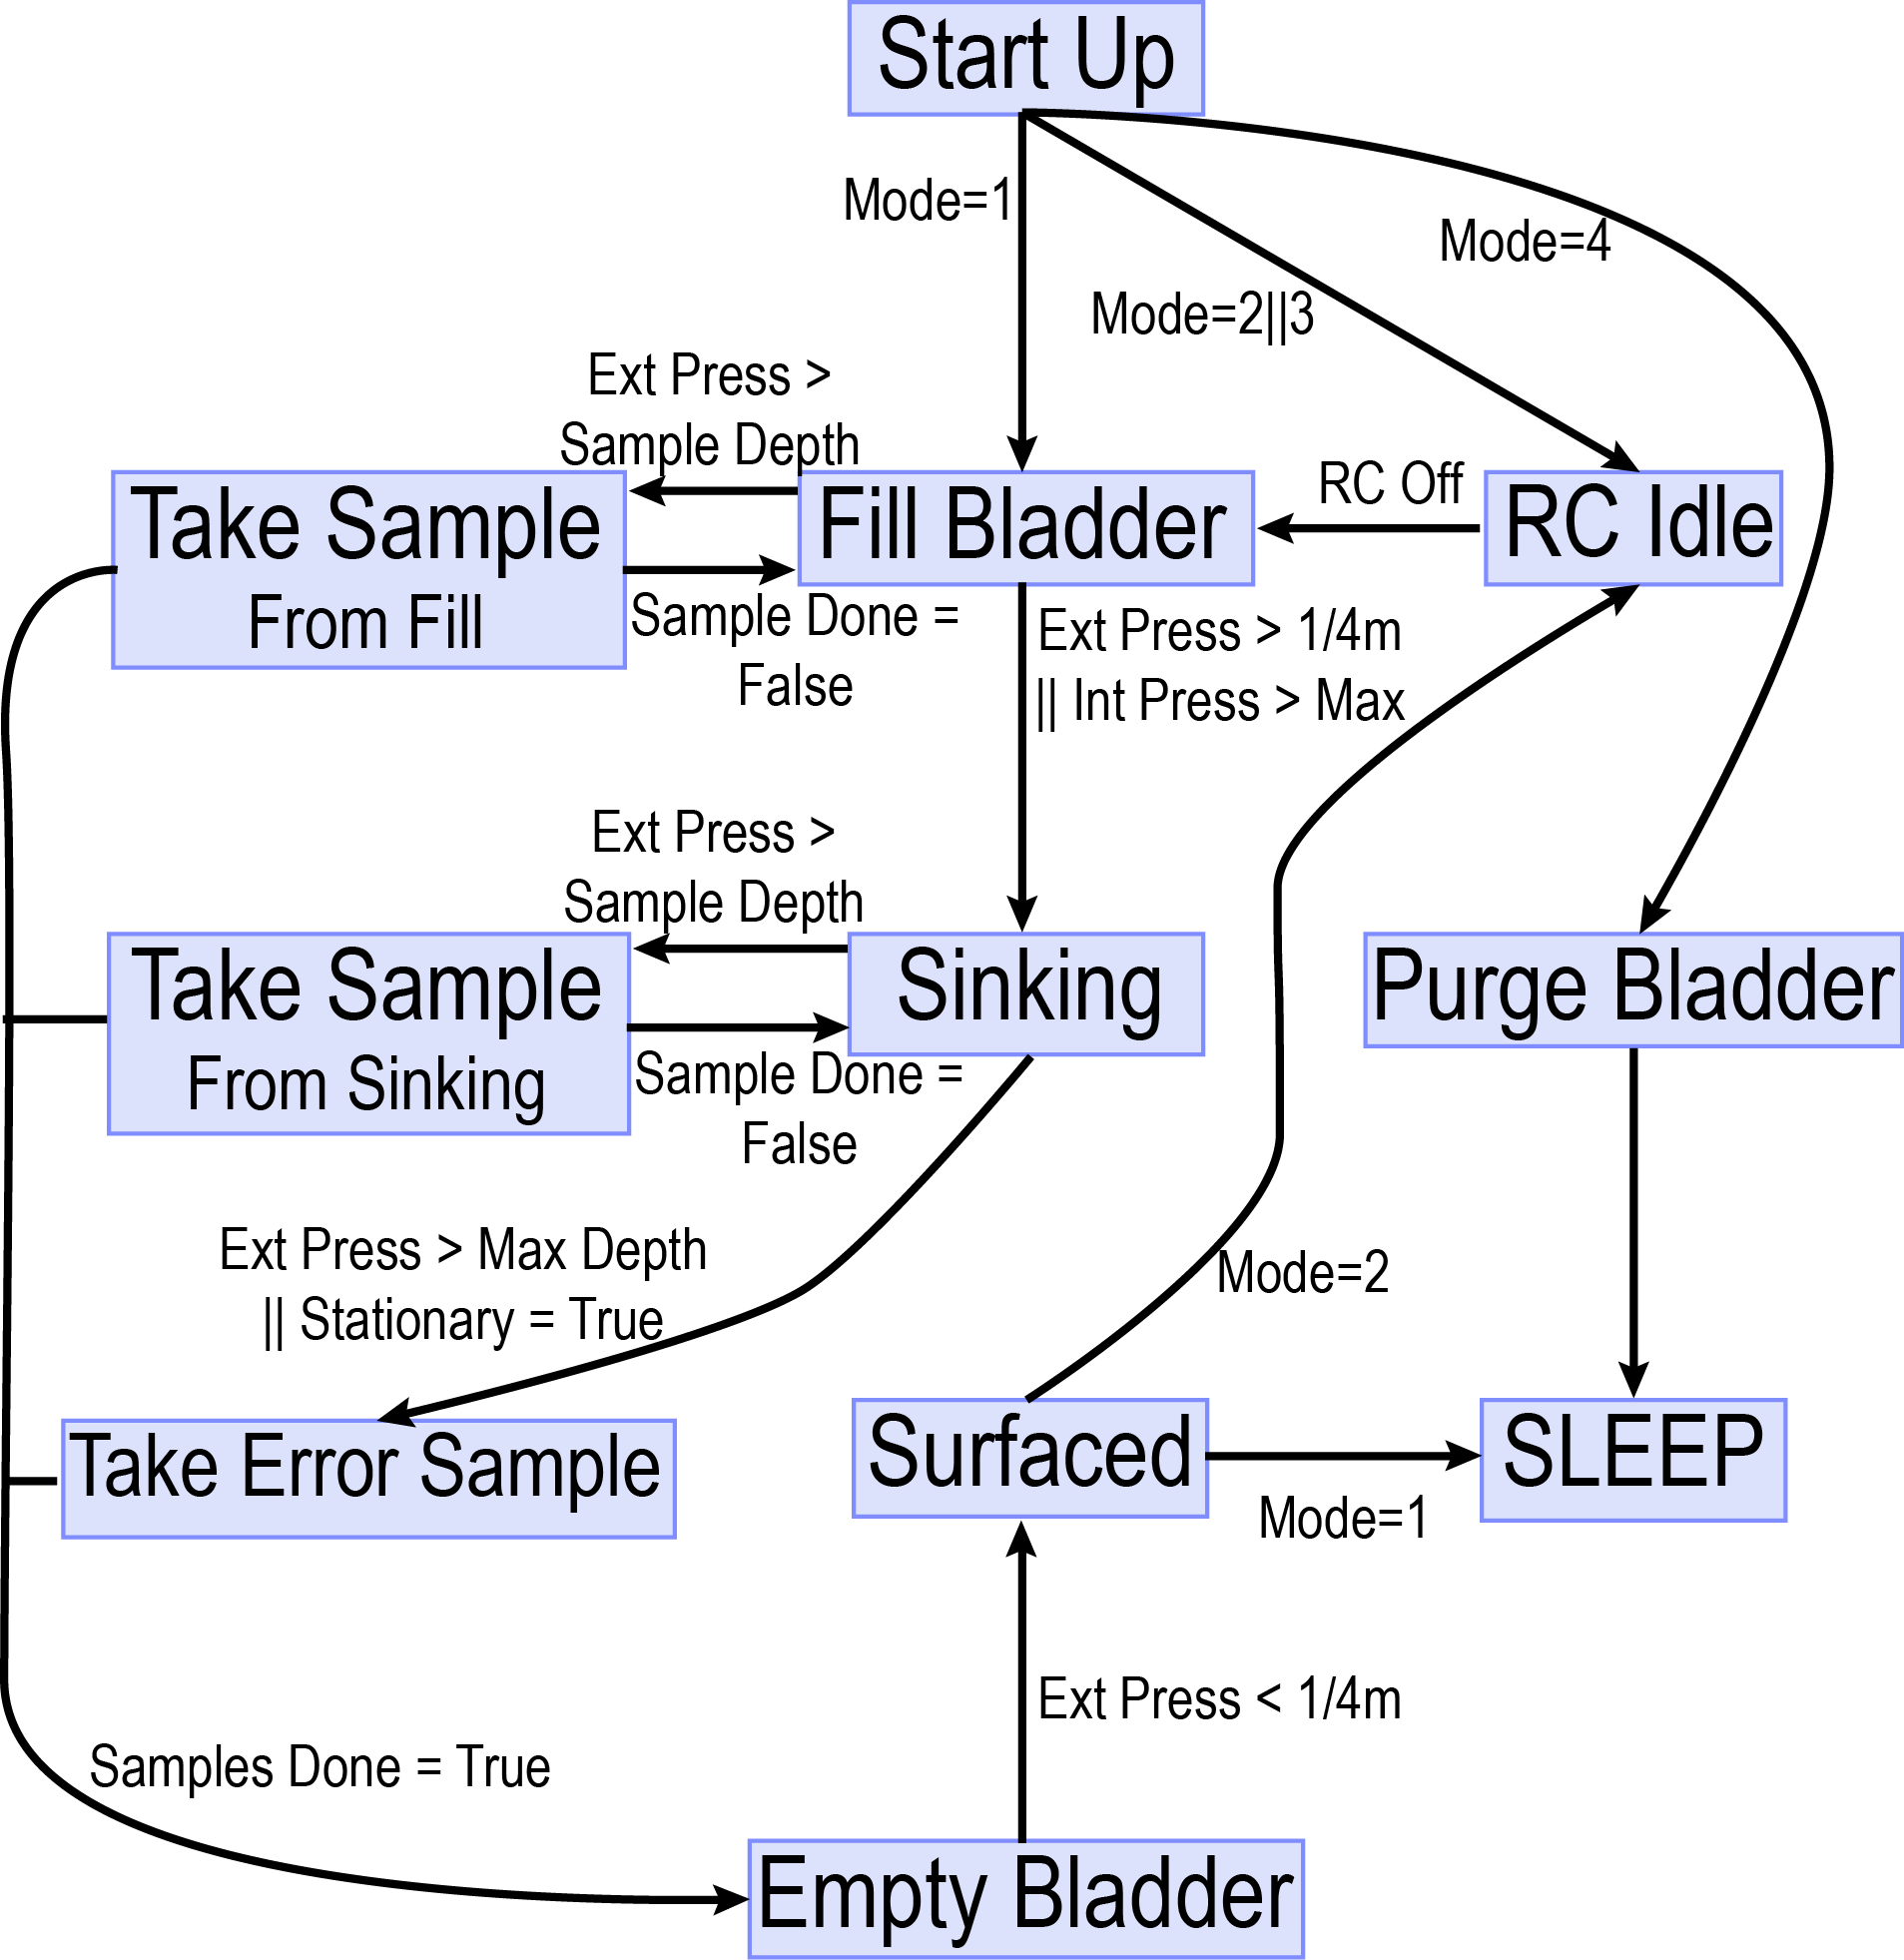
\includegraphics[width=1\columnwidth]{images/Statemachine.png}
	\caption{Aquapod state machine diagram}
	\vspace{-10pt}
	\label{fig:Statemachine}
\end{figure}

It was important to program a number of safety checks within the state machine to ensure that the robot will always resurface. Errors in the operation could include reaching a depth greater than 10m or hitting a surface before reaching the target depth. If one of these errors occurs, the robot will take a sample and return to the surface. Other system error checks were written directly into the slave board in case one of the boards reset, a sensor failure occurs, or other unlikely mishaps happen.

During either mode 2 or 3, the remote control (RC) operation is run. This allows the user to control the arms of the robot through a standard radio transmitter. In these modes the user can command the robot to tumbling to a particular location and dive or simply move around on land.

The state machine featured in Figure \ref{fig:Statemachine} is by no means extensive of the robot's capabilities. Further development and inclusion of the GPS module can greatly increase the functionality of the robot. This operation profile was simply used as an example for diving/sampling and as a demonstration tool. Autonomous control for long-term and unmonitored missions is feasible with the current hardware.

%%%%%%%%%%%%%%%%%%%%%%%%%%%%%%%%%%%%%%%%%%%%%%%%%%%%%%%%%%%%%%%%%%%%%%%%%%%%%%%%%%%%%%%%%%%%
\section{Experiments}
\label{experiments_aquapod}
To verify the mechanical design and embedded system programming, numerous experiments were carried out in a diving well. Figure \ref{fig:logfile} shows the results from a sample dive that was taken. The robot was programmed to take samples at 1m and 3m. The output log file includes the internal pressure values, depth in meters, the accelerometer sensors, temperature, and humidity. Markers are placed on the pressure graph to indicate event locations either the pump turning on or off(solid), or when a sample was taken(dotted).

%Pressure log file 
\begin{figure}[htb]
	\centering
	%\includegraphics[width=1\columnwidth]{images/testresults.png}
	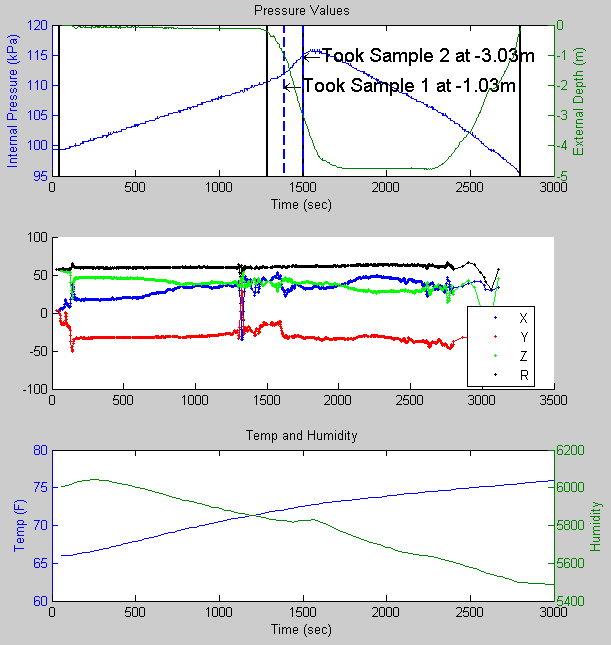
\includegraphics[width=1\columnwidth]{images/logfile.png}
	\caption{Experiment log file from an Aquapod dive}
	\vspace{-10pt}
	\label{fig:logfile}
\end{figure}

In addition to in-lab testing, the Aquapods were also brought to Houston for user testing with research biologists. The robots were demonstrated in several locations in marshlands near the coast including heavily vegetated and muddy environments. Feedback from this visit will be taken into consideration for future iterations of the Aquapod family.

%%%%%%%%%%%%%%%%%%%%%%%%%%%%%%%%%%%%%%%%%%%%%%%%%%%%%%%%%%%%%%%%%%%%%%%%%%%%%%%%%%%%%%%%%%%%
\subsection{Future Work}
%\label{future_work}
Though this iteration was a major improvement in functionality over the pervious RC Aquapod, many improvements are continously being explored to expand its capabilities. One area of continuing work for the Aquapod is communications. Currently the only method of communication is through hobby RC signals. However, Aquapods can be configured to carry distinct communication payloads, with each Aquapod serving as a node in a network that enables digital radio, cellular, and acoustic communications. 

Improvements to the electrical power system design include the use a single-cell LiPB. This broadens the range of compatible input power sources to include various energy harvesting modules - such as solar, wave, thermal, kinetic, etc.  Integrating dynamic power-path management into the charging circuit, in tandem with energy harvesting may also increase efficiency of energy use achieving overall gains in the robot's achievable runtime.

Another improvement relates to using the Aquapod for extended-period environmental monitoring. In this scenario, the robot collects relevant data in a manner that minimizes energy consumption for periods of 12 to 24 hours and then navigates to a waypoint for pickup.


%%%%%%%%%%%%%%%%%%%%%%%%%%%%%%%%%%%%%%%%%%%%%%%%%%%%%%%%%
\subsection{ Conclusions}

	The combination of the high terrainability, high mobility-to-size ratio, amphibious nature, and small size allows the deployment of the Aquapod in environments that would be difficult for most robots of the same size. The robot is designed to withstand water pressures up to 10 meters in depth, as well as be chemically compatible with the potential substances it may encounter.  The onboard embedded system was designed to perform as many modular expandable tasks in a limited amount of space, as well as provide intelligent power management to the system.  The redesign and further development of this robotic platform provided several advances in its capability for the specified environment of a shallow water marshland.
%%%%%%%%%%%%%%%%%%%%%%%%%%%%%%%%%%%%%%%%%%%%%%%%%%%%%%%%%